\documentclass[runningheads]{llncs}
\usepackage[T1]{fontenc}
\usepackage{graphicx}
\usepackage{amsmath}
\usepackage{amssymb}
\usepackage{booktabs}
\usepackage{svg}
\usepackage[misc]{ifsym}
\newcommand{\corr}{(\Letter)}
% N.B.: do not change anything above this line. If you require additional packages, please load them directly after this line.
\usepackage{mwe}
% N.B.: you may delete the preceding line. It is used to display an example image in this template.

\begin{document}

\title{Should We Compute Feature Effects on Training or Validation Data?}

% \titlerunning{Should We Compute Feature Effects on Training or Validation Data?}
% If the full title of your paper is short enough to also fit in the running head, you can omit the abbreviated paper title here. You can check as follows: if you comment out the \titlerunning line, something will appear in the header of all odd-numbered pages of your PDF from page 3 onward. This something is either the full title (in which case all is well), or the error message "Title Suppressed Due to Excessive Length". If this error message appears, you're going to want to provide an abbreviated title within the \titlerunning command, because if you won't do it, Springer will do it for you.

%N.B.: Author information (both in the \author{} and \authorrunning{} command) should only be present in the Camera-Ready Version of your paper. The version that you initially submit for review, ought to be double-blind. So, when initially submitting your paper, use:
%\author{Author information scrubbed for double-blind reviewing}
\author{Timo Heiß\inst{1}}
% You may leave out the orcidID information, if you want to.
% Use \corr to indicate the corresponding author. Note the spacing around the \corr command. Only one author can be the corresponding author.

%N.B.: comment out the \authorrunning{} command for the double-blind version of your paper submitted for review. Later, if your paper is accepted, use the command for the Camera-Ready Version.
\authorrunning{Timo Heiß}
% First names are abbreviated in the running head.
% If there is one author, write 'A.L. Benjamin'.
% If there are two authors, write 'A.L. Benjamin and C.C. Broadus Jr.'
% If there are more than two authors, '[...] et al.' is used.

\institute{Department of Statistics, LMU Munich, Ludwigstr. 33, 80539 Munich, Germany \email{t.heiss@campus.lmu.de}}

\maketitle              % typeset the header of the contribution

\begin{abstract}
    The abstract should briefly summarize the contents of the paper in
    150--250 words.

    \keywords{Explainable AI  \and Feature effects \and Partial dependence plot \and Accumulated local effects}
\end{abstract}

\section{Introduction}
Most Machine Learning (ML) models can be considered black boxes --- opaque
systems that intrinsically do not allow insight into their internal reasoning,
making it often impossible to explain their decisions. However, this can be
problematic in many domains and applications, such as the healthcare, legal, or
finance sectors, where decisions must be transparent and
accountable~\cite{adadi_peeking_2018}.

Interpretability is crucial to enhance
trust~\cite{ribeiro_why_2016,teach_analysis_1981}, address potential
biases~\cite{guidotti_survey_2019}, fairness and ethical concerns
~\cite{lipton_mythos_2018}, and ensure compliance with regulations such as the
EU's General Data Protection Regulation (GDPR)~\cite{gdpr2016} and AI
Act~\cite{euaia2024}. To address these challenges, the field of Explainable AI
/ Interpretable ML has emerged~\cite{adadi_peeking_2018}. Although there are
many different methods\footnote{For an overview of Explainable AI methods, see
    e.g.~\cite{adadi_peeking_2018,kamath_introduction_2021,molnar_interpretable_2022}.},
we will focus on feature effect methods like \textit{Partial Dependence Plots
    (PDP)}~\cite{friedman_greedy_2001} and \textit{Accumulated Local Effects
    (ALE)}~\cite{apley_visualizing_2020}.

Due to the severity of many applications, it is crucial to utilize these
explainability methods correctly. In general, there are many pitfalls to be
aware of~\cite{molnar_general_2022}, including whether to compute explanations
in-sample, i.e.\ on training data, or out-of-sample, which we refer to as
validation data in the following. In loss-based methods such as
\textit{Permutation Feature Importance (PFI)
}\cite{breiman_random_2001,fisher_all_2019}, this choice is crucial and has
already been studied (e.g., in~\cite{molnar_general_2022}). Nevertheless, other
explainability methods, such as the \textit{Mean Decrease in Impurity (MDI)}
(or \textit{Gini Importance}) of Random Forests, or \textit{SHAP}
values~\cite{loecher_debiasing_2022,loecher_debiasing_2024}, have also been
found to exhibit biases when computed on training data.

However, to the best of our knowledge, there exist no similar studies for
feature effect methods like PDP and ALE. Existing works, including the original
papers of PDP and ALE, rely on training data without further justification
(e.g.,~\cite{apley_visualizing_2020,friedman_greedy_2001,molnar_interpretable_2022}).
In contrast, practitioners often advocate for using unseen test/validation
data\footnote{see, e.g.\ \url{https://github.com/SauceCat/PDPbox/issues/68}
    (10/27/2024)}, or base their choice on practical constraints like dataset
size\footnote{see, e.g.
    \url{https://forums.fast.ai/t/partial-dependence-plot/98465} (10/27/2024)}.
While the training set is usually larger and might thus lead to less variance
in the feature effect estimates, a too large dataset can increase computation
times substantially, particularly for the PDP~\cite{friedman_greedy_2001}. On
the other hand, although feature effects are not based on generalization error
like PFI, it is not clear how much they are affected by overfitting or
distribution shifts between training and validation data.

In this paper, we aim to answer this largely unaddressed, fundamental
methodological question of whether to use training or validation data to
compute feature effects. We perform an empirical simulation study, comparing
feature effect error and uncertainty for PDP and ALE across training data,
validation data, and cross-validation scenarios, considering various data
scenarios and model types. Our main contributions in this paper are as follows.
\begin{enumerate}
    \item We shed light on the question of whether to compute feature effects on training
          data, validation data, or in a cross-validated manner, grounded through our
          comprehensive simulation study, considering feature effect error, bias, and
          variance across different models and data scenarios.
    \item We define methods to quantify feature effect error and uncertainty in a
          theoretical framework, building upon previous work in this area.
    \item We provide an overview of commonly used test functions for simulation studies
          in Interpretable ML, including applications and purposes.
\end{enumerate}

These contributions have several important implications: Our empirically
grounded recommendations enable practitioners and researchers to make informed
decisions about which dataset to select for feature effect computation, helping
to understand potential implications of their choices. Additionally, our
framework for evaluating feature effects and our systematic collection of test
functions provide a foundation for future research in Interpretable ML, with
the latter specifically facilitating test function choice for simulation
studies.

The remainder of this paper is structured as follows. In
\textsc{Section~\ref{sec:related-works}}, we introduce the considered feature
effect methods PDP and ALE, as well as related works on feature effect error
and uncertainty, and give an overview of common test functions for simulation
studies. In \textsc{Section~\ref{sec:quantify-fe-u}}, we extend existing works
and give our definitions of feature effect errors and uncertainty. We then
describe the methodology and set-up of our simulation studies in
\textsc{Section~\ref{sec:methodology-set-up}}, present the results in
\textsc{Section~\ref{sec:results}}, and discuss their implications and
limitations in \textsc{Section~\ref{sec:discussion}}. In
\textsc{Section~\ref{sec:conclusion}}, we briefly conclude our work.

\section{Background \& Related Work}\label{sec:related-works}

\subsection{Feature Effects}

The \textit{Partial Dependence Plot (PDP)} by
Friedman~\cite{friedman_greedy_2001} describes the marginal effect of one or
two features on the prediction of a model $\hat f$. For a feature set $X_S$
(with $S \subseteq \{1,\ldots,p\}$, $|S| = 1$ or $|S| = 2$), the PDP is defined
as

\begin{equation}
    PDP_{\hat f, S} = \mathbb{E}_{X_C}[\hat{f}(x_S, X_C)] = \int f(x_S, x_C)d\mathbb{P}(x_C),
\end{equation}

\noindent where $X_C$ is the complement feature subset. $PDP_{\hat f, S}$ is a
function of $x_S$ and can be estimated by Monte Carlo integration:

\begin{equation}\label{eq:pdp-estimate}
    \widehat{PDP}_{\hat f, S}(x_S) = \frac{1}{n} \sum_{i=1}^{n} \hat{f}(x_S, x_C^{(i)}).
\end{equation}

\noindent Here, $x_C^{(i)}$ are the actual complement feature values from the dataset of $n$ instances.
To plot this function, a grid of $G$ grid points
$\{(x_S^{(g)}, \widehat{PD}_{\hat f, S}(x_S^{(g)}))\}_{g=1}^G$ can be used~\cite{molnar_relating_2023}.
Molnar et al.~\cite{molnar_general_2022} recommend using quantile-based over equidistant grids.

The PDP assumes that the features in $S$ are independent of the features in
$C$. If this is violated, the perturbations may produce unrealistic data points
outside the underlying joint distribution of the data. This extrapolation issue
can cause misleading
interpretations~\cite{molnar_interpretable_2022,molnar_general_2022}.\\

\noindent The \textit{Accumulated Local Effects (ALE)} plot is an alternative to the PDP that
solves the extrapolation issue~\cite{apley_visualizing_2020}. Using the notation above,
for $|S|=1$, the ALE plot is defined as

\begin{eqnarray}
    ALE_{\hat f,S}(x_S) &=& \int_{x_{\text{min},s}}^{x_S} \mathbb{E}_{X_C|X_S}
    \left[\hat{f}^S(X_S, X_C)|X_S = z_S\right] dz_S - \text{constant} \\
    &=& \int_{x_{\text{min},s}}^{x_S} \int_{x_C}
    \hat{f}^S(z_S, x_C)\mathbb{P}(x_C|z_S)dx_{C}dz_{S} - \text{constant},
\end{eqnarray}

\noindent where $\hat{f}^S(x_S, x_C) = \frac{\partial \hat{f}(x_S, x_C)}{\partial x_S}$.
The constant is chosen so that $\widehat{ALE}_{\hat f,S}(X_S)$ is centered with a mean of $0$
w.r.t.\ the marginal distribution of $X_S$. The uncentered ALE can be estimated by

\begin{equation}\label{eq:ale-estimate-uncentered}
    \widehat{\widetilde{ALE}}_{\hat f, S}(x) =
    \sum_{k=1}^{k_S(x)} \frac{1}{n_S(k)} \sum_{i:x_S^{(i)} \in N_S(k)}
    \left[\hat f(z_{k,S}, x_{C}^{(i)}) - \hat f(z_{k-1,S}, x_{C}^{(i)})\right].
\end{equation}

\noindent Here, $\{N_S(k) = (z_{k-1,S}, z_{k,S}]\}_{k=1}^{K}$ partitions the samples
$\{x^{(i)}_S\}_{i=1}^n$ into $K$ intervals or neighborhoods $N_S(k)$. $n_S(k)$ denotes
the number of observations in the $k$th interval $N_S(k)$, $k_S(x)$ represents the index
of the interval to which a particular value $x$ of feature $x_S$ belongs.
The uncentered ALE is centered by

\begin{equation}\label{eq:ale-estimate-centered}
    \widehat{ALE}_{\hat f, S}(x) =
    \widehat{\widetilde{ALE}}_{\hat f, S}(x)
    - \frac{1}{n} \sum_{i=1}^n \widehat{\widetilde{ALE}}_{\hat f, S}(x_S^{(i)})
\end{equation}

\noindent to have a mean effect of $0$. For the grid that defines the intervals,
the quantiles of the empirical distribution of $\{x^{(i)}_S\}_{i=1}^n$ can be
used~\cite{apley_visualizing_2020}.\\

\noindent Other feature effect methods include the \textit{M-Plot (Marginal Plot)},
which, however, suffers from the omitted variable
bias~\cite{apley_visualizing_2020,friedman_greedy_2001},
or \textit{functional ANOVA (fANOVA)}, which decomposes feature effects
into main and interaction effects~\cite{hooker_discovering_2004}.

Furthermore, methods exist that extend previous ones, such as \textit{Robust
    and Heterogeneity-aware ALE (RHALE)}~\cite{gkolemis_rhale_2023}, or
\textit{Accumulated Total Derivative Effect (ATDEV)} plots, which can be
decomposed into ALE and \textit{Accumulated Cross Effects
    (ACE)}~\cite{liu_model_2018}.

In addition to these global feature effect methods, there are regional effect
plots such as \textit{REPID}~\cite{herbinger_repid_2022}, as well as local
methods, including \textit{ICE (Individual Conditional Expectation)}
curves~\cite{goldstein_peeking_2015} or SHAP dependence plots
(e.g.,~\cite{molnar_interpretable_2022}) based on SHAP
values~\cite{lundberg_unified_2017}.

For the remainder of this paper, we will focus on PDP and ALE as the most
popular global feature effect methods and refer to them when speaking of
feature effects.

\subsection{Feature Effect Error Decomposition}

To quantify the error of a computed feature effect, a ``ground truth'' needs to
be defined first. We follow the approach of Molnar et
al.~\cite{molnar_relating_2023} and define ground truth versions of PDP and ALE
directly on the data generating process (DGP) by applying PDP and ALE to the
underlying ground truth function $f$ (instead of model $\hat f$).

For PDP, we can directly use the definition of Molnar et
al.~\cite{molnar_relating_2023}:

\begin{definition}[Definition 1 from~\cite{molnar_relating_2023}]
    The PDP ground truth is the PDP applied to function
    $f : \mathcal{X} \xrightarrow{} \mathcal{Y}$
    of the data generating process.

    \begin{equation}
        PDP_{f,S}(x_S) = \mathbb{E}_{X_C}[f(x_S,X_C)]
    \end{equation}
\end{definition}

As stated by Molnar et al.~\cite{molnar_relating_2023}, their results also
apply to conditional variants of the PDP such as ALE. We now make this
definition explicit:

\begin{definition}
    The ALE ground truth is the ALE applied to function $f : \mathcal{X} \xrightarrow{} \mathcal{Y}$ of the data generating process.

    \begin{equation}
        ALE_{f,S}(x_S) = \int_{x_{\text{min},s}}^{x_S} \mathbb{E}_{X_C|X_S} \left[f^S(X_S, X_C)|X_S = z_S\right] dz_S - \text{constant}
    \end{equation}

    \noindent where $f^S(x_S, x_C) = \frac{\partial f(x_S, x_C)}{\partial x_S}$ and \text{constant} chosen such that the effect has a mean of $0$ w.r.t. the marginal distribution of $X_S$.
\end{definition}

%With these definitions, $\widehat{PDP}_{\hat f,S}$ and $\widehat{ALE}_{\hat f,S}$
%can now be treated as statistical estimators of the ground truth feature effects
%(cf.~\cite{molnar_relating_2023}). 
Note that different ground truth effects may also be defined, and our choices
come with certain implications and limitations, such as omitting the
\textit{aggregation bias}\footnote{for details,
    see~\cite{herbinger_repid_2022}}~\cite{mehrabi_survey_2021}.

With more complex ground truth functions $f$, it may become increasingly
difficult to derive the ground truth feature effects analytically, especially
for ALE. In these cases, we therefore propose to also estimate those effects by
Monte Carlo integration, yielding $\widehat{PDP}_{f,S}(x_S)$ and
$\widehat{ALE}_{f,S}(x_S)$ (obtained by plugging in $f$ instead of $\hat f$
into the estimators in equations (\ref{eq:pdp-estimate}) and
(\ref{eq:ale-estimate-uncentered}) / (\ref{eq:ale-estimate-centered})).\\

\noindent Summarizing, we have now defined four quantities per feature effect:
$PDP_{f,S}$ $\widehat{PDP}_{f,S}$, $PDP_{\hat f,S}$, and $\widehat{PDP}_{\hat f,S}$
(analogue for ALE). We can now define different errors between each of these
quantities. In this paper, we focus on the MSE, as it can be decomposed into
bias and variance (see e.g.~\cite{geman_neural_1992}).
Taking, for example, $PDP_{f,S}$ as ground truth, we can define the MSE of
$PDP_{\hat f,S}$ at a point $x_S$ as follows~\cite{molnar_relating_2023}:

\begin{equation}
    \text{MSE}(x_S; PDP_{f,S}, PDP_{\hat f,S})
    = \mathbb{E}_F[{(PDP_{f,S}(x_S) - \widehat{PDP}_{\hat f,S}(x_S))}^2]
\end{equation}
\begin{equation}
    = \underbrace{{(PDP_{f,S}(x_S) - \mathbb{E}_F[PDP_{\hat{f},S}(x_S)])}^2}_{Bias^2} + \underbrace{\text{Var}_F[PDP_{\hat{f},S}(x_S)]}_{Variance}
\end{equation}

\noindent Here, $F$ denotes the distribution of trained models. The bias
is linked to the bias of the model, the variance comes from the variance
in the model fits (randomness in training data, randomness in model training procedure).

Since we usually cannot determine $PDP_{\hat f,S}$, we need to estimate it by
Monte Carlo integration, yielding $\widehat{PDP}_{\hat f,S}(x_S)$. This,
however, introduces an additional variance term (we use the random variable
$X_{mc}$ for the Monte Carlo samples (e.g., training or validation data)):

\begin{equation}
    \begin{split}
        \text{MSE}(x_S; PDP_{f,S}, \widehat{PDP}_{\hat f,S})
        = \underbrace{{(PDP_{f,S}(x_S) - \mathbb{E}_F[PDP_{\hat{f}, S}(x_S)])}^2}_{Bias^2} \\
        + \underbrace{\text{Var}_F[PDP_{\hat{f},S}(x_S)]}_{Variance} + \underbrace{\mathbb{E}_F\text{Var}_{X_{mc}}[\widehat{PDP}_{\hat{f},S}(x_S)]}_{MC-Variance}
    \end{split}
\end{equation}

\begin{proof}
    For better readability, we will omit the subscript $S$ as well as the point $x_S$ and use $X=X_{mc}$ in this proof:

    \begin{align*}
        \text{MSE}(PDP_{f}, \widehat{PDP}_{\hat f})
         & = \mathbb{E}_F\mathbb{E}_X[(PDP_f - \widehat{PDP}_{\hat f})^2]                                                                                         \\
         & = \mathbb{E}_F \mathbb{E}_X[PDP_f^2 - 2PDP_f\widehat{PDP}_{\hat f} + \widehat{PDP}_{\hat f}^2]                                                         \\
         & = PDP_f^2 - 2PDP_f\mathbb{E}_F[PDP_{\hat f}] + \mathbb{E}_F\mathbb{E}_X[\widehat{PDP}_{\hat f}^2]                                                      \\
         & = PDP_f^2 - 2PDP_f\mathbb{E}_F[PDP_{\hat f}] + \mathbb{E}_F\text{Var}_X[\widehat{PDP}_{\hat f}] + \mathbb{E}_F[\mathbb{E}_X[\widehat{PDP}_{\hat f}]^2] \\
         & = PDP_f^2 - 2PDP_f\mathbb{E}_F[PDP_{\hat f}] + \mathbb{E}_F\text{Var}_X[\widehat{PDP}_{\hat f}] + \text{Var}_F(\mathbb{E}_X[\widehat{PDP}_{\hat f}])   \\
         & \quad + \mathbb{E}_F(\mathbb{E}_X[\widehat{PDP}_{\hat f}])^2                                                                                           \\
         & = PDP_f^2 - 2PDP_f\mathbb{E}_F[PDP_{\hat f}] +  Var_F[PDP_{\hat f}] + \mathbb{E}_F[PDP_{\hat f}]^2 + \mathbb{E}_F\text{Var}_X[\widehat{PDP}_{\hat f}]  \\
         & = (PDP_f - \mathbb{E}_F[PDP_{\hat f}])^2 + \text{Var}_F[PDP_{\hat f}] + \mathbb{E}_F[\text{Var}_X(\widehat{PDP}_{\hat f})]
    \end{align*}

    \noindent At multiple points, we use the fact that $\mathbb{E}_X[\widehat{PDP}_{\hat f}]
        = PDP_{\hat f}$ (cf.~\cite{molnar_relating_2023}).
\end{proof}

\noindent We see that the variance due to MC integration also depends on the model
distribution $F$. Similarly, one could use the estimate $\widehat{PDP}_{f,S}$
as groundtruth, introducing an additional variance term $Var_{X_{mc2}}$when
estimated on different MC sample (proof in
\textsc{Appendix~\ref{app:proof-mc-variance}}).
An overview of all error terms in this chian can be found in
\textbf{Fig.\@~\ref{fig:error-graph}}.\\

\begin{figure}[t]
    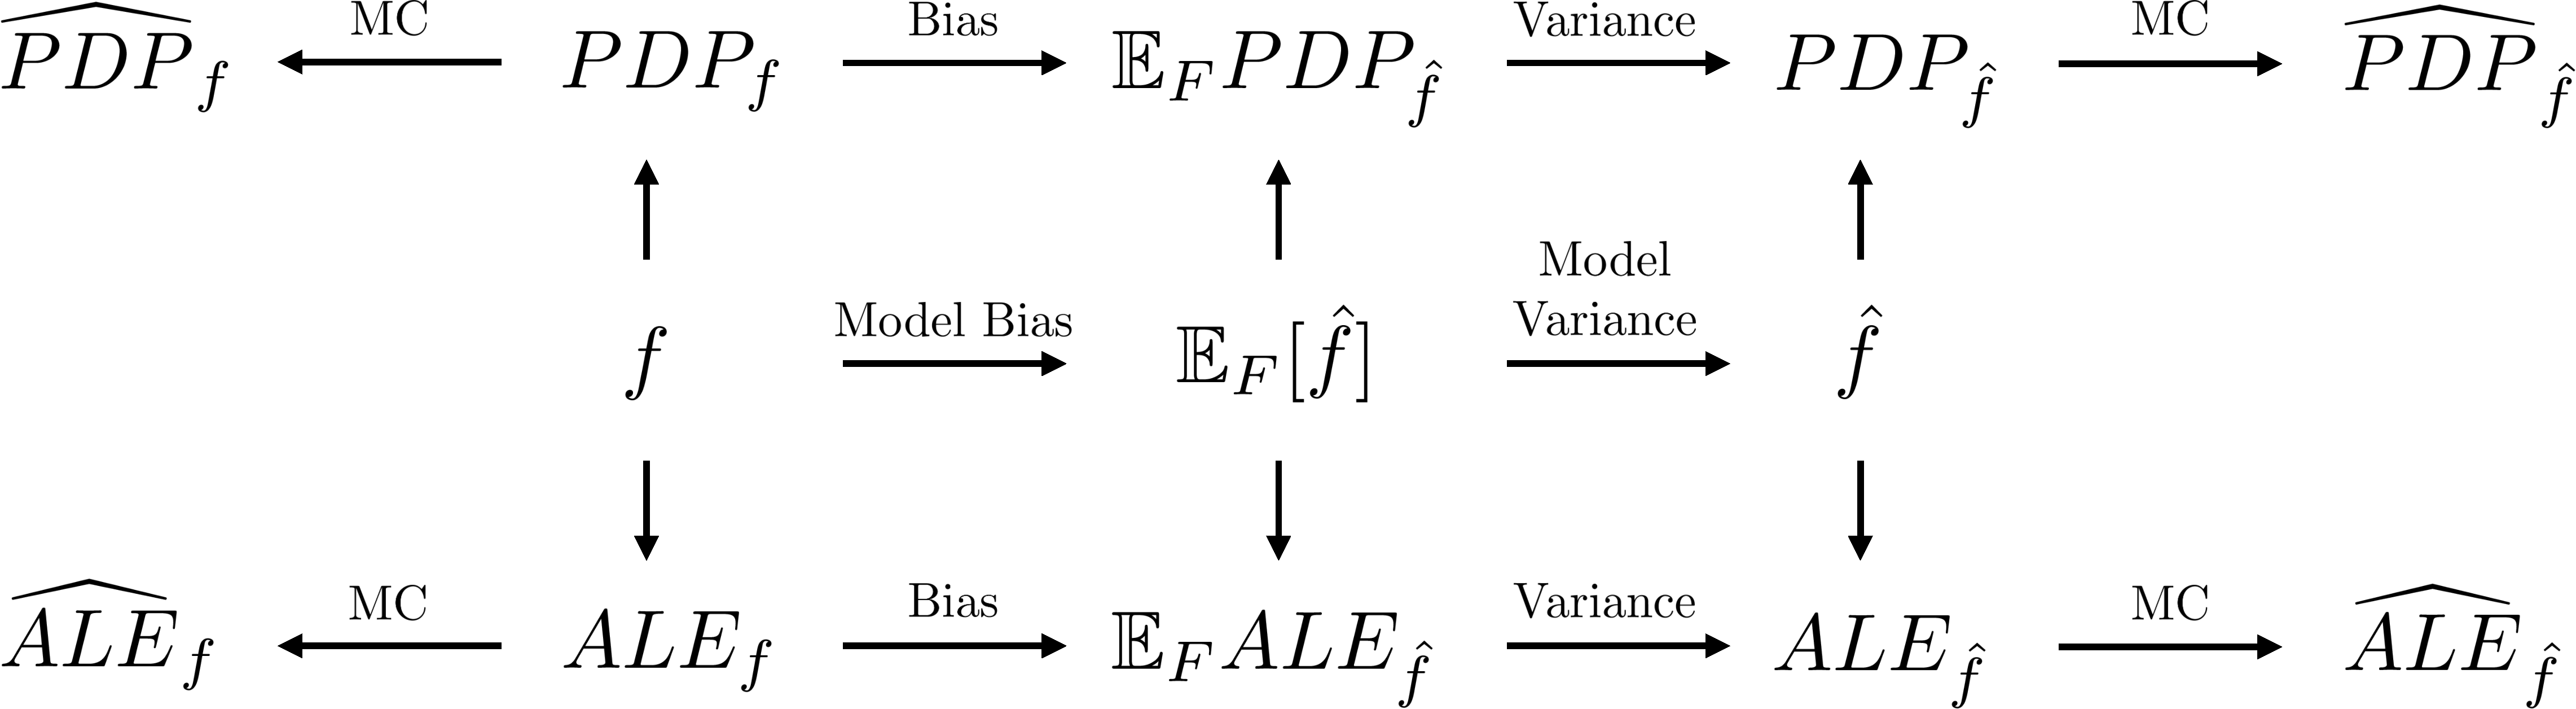
\includegraphics[width=\textwidth]{img/error_graph.pdf}
    \caption{Error chain in feature effect estimation
        (modified, original version can be found in~\cite{molnar_relating_2023})}\label{fig:error-graph}
\end{figure}

\noindent $\mathbb{E}_F$ and $\text{Var}_F$ could be estimated by averaging over
multiple models of the same inducer fitted to $M$ different training data
sets sampled independently from the DGP. We propose the following estimators:
\begin{equation}
    \widehat{\text{MSE}}(x_S; PDP_{f,S}, \widehat{PDP}_{\hat f,S}) = \frac{1}{M} \sum_{m=1}^{M} {(PDP_{f,S}(x_S) - \widehat{PDP}_{\hat f^{(m)},S}(x_S))}^2
\end{equation}
\begin{equation}
    \widehat{\text{Bias}}(x_S; PDP_{f,S}, \widehat{PDP}_{\hat f,S}) = (PDP_{f,S}(x_S) - \frac{1}{M}\sum_{m=1}^M \widehat{PDP}_{\hat{f}^{(m)},S}(x_S))
\end{equation}
\begin{equation}
    \widehat{\text{Variance}}(x_S; \widehat{PDP}_{\hat f,S}) =
    \frac{1}{M-1}\sum_{m=1}^M\left(\widehat{PDP}_{\hat f^{(m)},S}(x_S) - \frac{1}{M}\sum_{m=1}^M \widehat{PDP}_{\hat f^{(m)},S}(x_S)\right)^2
\end{equation}

\noindent Note that these are similar to the approach in~\cite{molnar_relating_2023},
but we do not specify which data points to use for MC integration. The
variance captures both the variance in the model fits and the variance due to
MC integration. To estimate the MC variance, we propose the following estimators:
\begin{equation}
    \widehat{\text{Variance}}_{MC}(x_S; PDP_f, \widehat{PDP}_f) = \frac{1}{K}\sum_{k=1}^K(PDP_f(x_S) - \widehat{PDP}_f^{(k)}(x_S))^2
\end{equation}

and
\begin{equation}
    \begin{split}
        \widehat{\text{Variance}}_{MC}(x_S; \widehat{PDP}_{\hat{f}}) = \\ \frac{1}{M(K-1)}\sum_{m=1}^M \sum_{k=1}^K
        \left(\widehat{PDP}_{\hat f^{(m)},S}^{(k)}(x_S) - \frac{1}{K}\sum_{k=1}^K \widehat{PDP}_{\hat f^{(m)},S}^{(k)}(x_S)\right)^2
    \end{split}
\end{equation}

\noindent For more convenient analysis of the errors, one could also
aggregate them over the marginal distribution of $X_S$ (e.g.,
estimated by averaging over the grid points if chosen appropriately)
to obtain a single error measure per feature effect.

While our definitions are based on the PDP, they can be directly applied to the
ALE as well.

\section{Test Functions for Simulation Studies}\label{sec:test-functions}

Test functions play a crucial role in research, e.g.\ for evaluating and
comparing different methodological approaches, or when conducting simulation
studies. This section synthesizes commonly used test functions across various
domains, providing structured guidance for researchers --- particularly those
in Interpretable ML --- in selecting appropriate test functions for their
simulation studies. By examining test functions from different fields and their
purposes of application, we aim to facilitate experimental design decisions.
While this overview is not exhaustive, it highlights key test functions and
their characteristics to help researchers make informed choices for their
specific research needs.

\paragraph{Test Functions in Optimization.}
The field of optimization, where test functions are essential to enable the
assessment and comparison of optimization algorithms, has established a rich
foundation of test functions. A fundamental approach involves using simple
mathematical expressions like the sphere function~\cite{more_testing_1981}.
These basic functions are often combined with more complex ones like Branin or
Rosenbrock to create comprehensive test suites that incorporate important
properties such as nonlinearity, non-separability, and
scalability~\cite{whitley_building_1998}. A notable framework in this domain is
the Comparing Continuous Optimizer (COCO) platform with its Black Box
Optimization Benchmark (BBOB), offering a structured approach to testing
continuous optimization algorithms through artificial test
functions~\cite{hansen_coco_2016}. These classical test function suites are
well-established in optimization and may also serve as a basis for
Interpretable ML researchers. However, it is important to note that the ability
of these artifical test functions to represent complex real-world behavior is
limited~\cite{zaefferer_simulation-based_2017}.

\paragraph{Physics-Inspired Test Functions.}

Physics-derived functions offer a compelling source of real-world test cases,
with the Feynman Symbolic Regression Database (FSReD) being a prominent
example. FSReD comprises 100 physics equations from the seminal
\textit{Feynman's Lectures on Physics (34--36)}, supplemented by 20 more
challenging equations from other seminal physics texts~\cite{udrescu_ai_2020}.
These equations span diverse physics domains including classical mechanics,
electromagnetism, and quantum mechanics. They involve between one and nine
independent variables and incorporate various elementary functions such as
arithmetic operations, trigonometric functions, and exponentials. From that,
tabular datasets were generated through random sampling from defined value
ranges.

Building upon this foundation,
Matsubara~et~al.~\cite{matsubara_rethinking_2024} addressed several limitations
of the original FSReD. Their enhanced framework introduces a three-tiered
categorization of problems (easy, medium, hard) based on their complexity,
incorporates dummy variables to simulate irrelevant features, and implements
more realistic sampling ranges and strategies. Detailed specifications for all
formulas, including their sampling parameters, are available in their work.

While initially developed for symbolic regression tasks, many Feynman equations
may serve as suitable test functions for simulation studies in Interpretable
ML. Their basis in physical principles provides real-world relevance, though
researchers should carefully select equations that align with their specific
analytical objectives and complexity requirements.

\paragraph{Test Functions for Interpretable Machine Learning.}
The Interpretable ML field itself has developed several specialized test
functions designed to evaluate specific aspects of interpretability methods.

Goldstein et al.~\cite{goldstein_peeking_2015} used several simple test
functions to demonstrate the behavior of Individual Conditional Expectation
(ICE) curves. These include a simple additive function to demonstrate the
absence of interactions, simple interactions to reveal heterogeneity that might
be obscured by averaging procedures such as PDPs, and a specially designed
function with an empty quadrant for assessing extrapolation behavior.

Similarly, Liu et al.~\cite{liu_model_2018} focus on simple functions before
progressing to more complex ones. They begin with basic two-variable scenarios
--- using additive functions, interaction functions, and combinations thereof
--- and examine these under both independent and correlated feature conditions
to compare various feature effect methods. The advantage of these simple test
functions is that solutions (e.g., feature effects) can also be computed
analytically, and that they allow for deeper and more fine-grained analysis of
individual aspects.

A more complex test function suite was proposed by
Tsang~et~al.~\cite{tsang_detecting_2017}, specifically designed to evaluate the
detection of variable interactions. Their functions incorporate various types
of interactions with different orders, strengths, non-linearities, and
overlaps. While this makes them particularly valuable for interaction
detection, they are also useful for evaluating other interpretability methods
in scenarios with complex interactions.

The Friedman functions~\cite{breiman_bagging_1996,friedman_multivariate_1991}
serve as classical benchmarks applicable across various interpretability tasks.
These three functions combine linear and non-linear effects with interactions,
incorporating dummy variables and random noise terms to reflect realistic
complexity. For detailed specifications, see~\cite{breiman_bagging_1996}.

When choosing test functions for simulation studies in Interpretable ML,
researchers should consider several criteria, including the specific aspects of
interpretability being evaluated, the desired complexity level and number of
variables, the presence of specific challenges such as correlation between
features or interactions, the need for analytical solutions for validation, as
well as the relevance to real-world applications in the domain of interest.

\section{Methodology \& Experimental Set-Up}\label{sec:methodology-set-up}

\section{Results}\label{sec:results}

\section{Discussion}\label{sec:discussion}

\section{Conclusion}\label{sec:conclusion}

% \begin{table}[t]
% \caption{Table captions should be placed above the
% tables.}\label{tab1}
% \begin{tabular}{lll}
% \toprule
% Heading level &  Example & Font size and style\\
% \midrule
% Title (centered) &  {\Large\bfseries Lecture Notes} & 14 point, bold\\
% 1st-level heading &  {\large\bfseries 1 Introduction} & 12 point, bold\\
% 2nd-level heading & {\bfseries 2.1 Printing Area} & 10 point, bold\\
% 3rd-level heading & {\bfseries Run-in Heading in Bold.} Text follows & 10 point, bold\\
% 4th-level heading & {\itshape Lowest Level Heading.} Text follows & 10 point, italic\\
% \bottomrule
% \end{tabular}
% \end{table}

\begin{credits}
    \subsubsection{\ackname} A bold run-in heading in small font size at the end of the paper is used for
    general acknowledgments, for example: This study was funded by X (grant number
    Y).

    \subsubsection{\discintname}
    The authors have no competing interests to declare that are relevant to the
    content of this article.
\end{credits}

%
% ---- Bibliography ----
\bibliographystyle{splncs04}
\bibliography{mybibliography}

% appendix
\newpage
\appendix
\section{Proof: Monte Carlo Variance for Groundtruth}\label{app:proof-mc-variance}
\begin{proof}
    For better readability, we will omit the subscript $S$ as well as the point $x_S$ and use $X=X_{mc}$ in this proof:

    \begin{align*}
        \mathbb{E}_F\mathbb{E}_X[(PDP_f - \widehat{PDP}_f)^2] & = \mathbb{E}_F\mathbb{E}_X[PDP_f^2 - 2PDP_f \widehat{PDP}_f + \widehat{PDP}_f^2]                                 \\
                                                              & = PDP_f^2 - 2PDP_f \mathbb{E}_F\mathbb{E}_X[\widehat{PDP}_f] + \mathbb{E}_F\mathbb{E}_X[\widehat{PDP}_f^2]       \\
                                                              & = PDP_f^2 - 2PDP_f^2 + \mathbb{E}_F\text{Var}_X[\widehat{PDP}_f] + \mathbb{E}_F[\mathbb{E}_X[\widehat{PDP}_f]^2] \\
                                                              & = PDP_f^2 - 2PDP_f^2 + \mathbb{E}_F\text{Var}_X[\widehat{PDP}_f] + PDP_f^2                                       \\
                                                              & = \mathbb{E}_F\text{Var}_X[\widehat{PDP}_f]                                                                      \\
                                                              & = \text{Var}_X[\widehat{PDP}_f]
    \end{align*}

    \noindent Again we use $\mathbb{E}_X[\widehat{PDP}_{f}] = PDP_{f}$ (cf.~\cite{molnar_relating_2023}) as well as the fact
    that all quantities based on $f$ do not depend on the model distribution $F$.
\end{proof}

\end{document}
